\documentclass[a4paper,11pt,cours]{nsi} % COMPILE WITH DRAFT
\geometry{margin=2cm}
\usepackage[]{fontawesome5}
\usetikzlibrary{trees}

\setcounter{chapter}{2} % 1 de moins que le num de chapitre

\setlength{\columnseprule}{0pt}
\setlength{\columnsep}{1cm}

\chapter{Lois discrètes}

\begin{document}

\section{Rappels sur les variables aléatoires}
\begin{definition}[ : espérance, variance et écart-type]
	Soit $X$ une variable aléatoire dont la loi de probabilité est résumée dans le tableau ci-dessous:
	\begin{center}
		\colorbox{white}{
			\begin{tabular}{|l|c|c|c|c|}
				\hline
				\textbf{{\boldmath Valeur de $X$}} & $x_1$ & $x_2$ & $\cdots$ & $x_n$\\
				\hline
				{\boldmath $P(X=x_i)$} & $p_1$ & $p_2$ & $\cdots$ & $p_n$\\
				\hline
		\end{tabular}}
	\end{center}
	
	\begin{enumerate}[label=\textbullet]
		\item	L'\textbf{{\boldmath espérance de $X$}} est le nombre noté {\boldmath $E(X)$} défini par:\\
		\centerline{{\boldmath $E(X)=p_1 x_1+p_2 x_2+\ldots+p_n x_n$}} 
		noté aussi {\boldmath $E(X)=\displaystyle \sum_{i=1}^{n} p_i x_i$}.
		\item La 	\textbf{{\boldmath variance de $X$}} le nombre noté {\boldmath $V(X)$} défini par:\\
		\centerline{{\boldmath $V(X)=p_1 \left(x_1-E(X)\right)^2+p_2 \left(x_2-E(X)\right)^2+\ldots+p_n \left(x_n-E(X)\right)^2$}}
		noté aussi {\boldmath $V(x)=\displaystyle \sum_{i=1}^{n} p_i\left(x_i-E(X)\right)^2$}.
		\item  L'\textbf{{\boldmath écart-type de $X$}} le nombre noté {\boldmath $\sigma(X)$} défini par: {\boldmath $\sigma(X)=\sqrt{V(X)}$}.
	\end{enumerate}
\end{definition}

\begin{propriete}[]
	\begin{enumerate}[label=\textbullet]
		\item 	On a aussi: {\boldmath $V(X)=E(X^2)-[E(X)]^2$}.
		\item 	Soit $a$ et $b$ deux réels. Alors: {\boldmath $\quad E(aX+b)=aE(X)+b\quad$ et 							$\quad V(aX)=a^2 V(X)$}.
	\end{enumerate}
\end{propriete}

\subsection*{Interprétation de l'espérance et de l'écart-type}
Lors d'un jeu, l'\textbf{espérance de gain} représente le \textbf{gain moyen} que peut espérer le joueur lors d'un grand nombre de parties.
\begin{itemize}
	\item 	Si ce gain moyen est \textbf{nul}, on dit que le jeu est \textbf{équitable}.
	\item 	Si ce gain moyen est \textbf{positif}, on dit que le jeu est \textbf{favorable} au joueur
	\item 	Si ce gain moyen est \textbf{négatif}, on dit que le jeu est \textbf{défavorable} au joueur.
\end{itemize}
L'\textbf{écart-type du gain} mesure la \textbf{dispersion} des gains autour du gain moyen.\\
Plus l'écart-type est grand, plus la variable aléatoire est dispersée et plus le degré de risque du jeu est grand.

\begin{encadrecolore}{Rappels sur les probabilités conditionnelles}{UGLiBlue}
	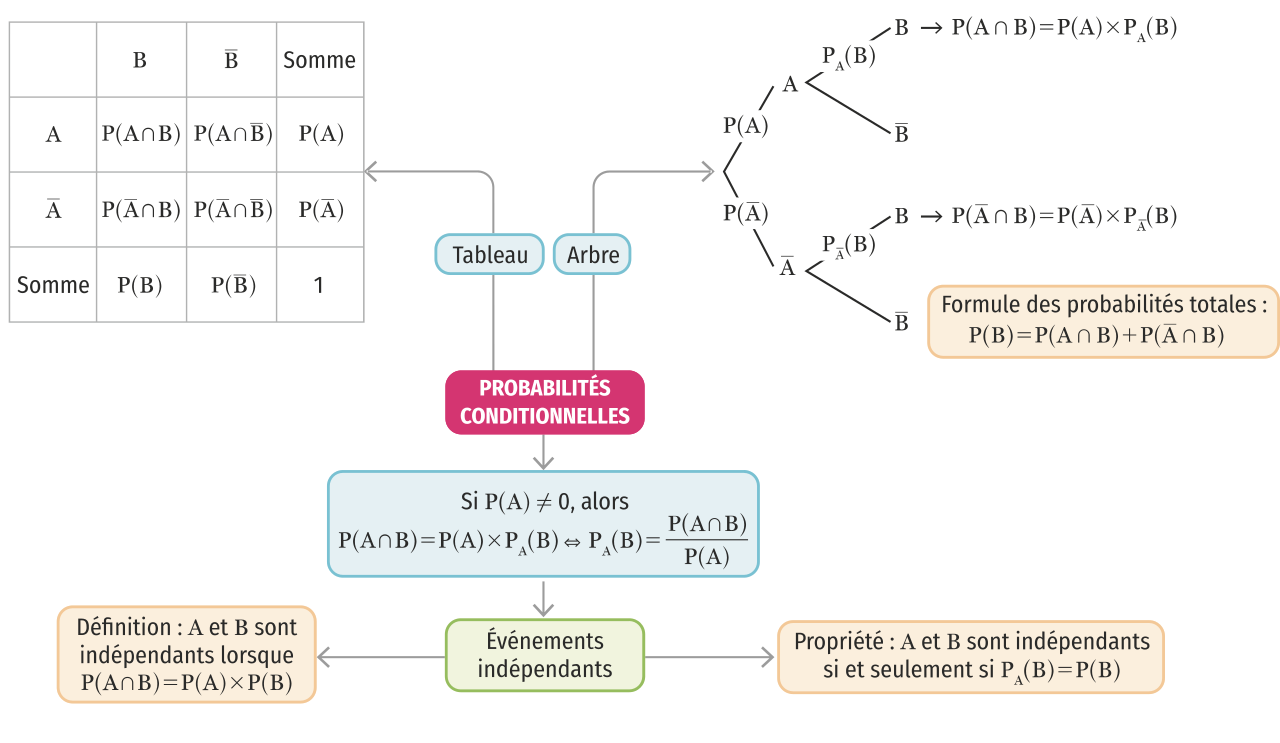
\includegraphics[width=16.5cm]{cartementale}
\end{encadrecolore}


\section{Loi uniforme sur $\left\{1\ ; 2\ ; ... \ ; n\right\}$}
\begin{definition}[]
    Soit $n$ un entier strictement positif.\\
    Une variable aléatoire $X$ suit la \textbf{loi uniforme sur $\left\{1\ ; 2\ ; ... \ ; n\right\}$} si elle prend pour valeurs les entiers de $1$ à $n$ de manière équiprobable.\\[.5em]
    Autrement dit, une variable aléatoire $X$ suit la \textbf{loi uniforme sur $\left\{1\ ; 2\ ; ... \ ; n\right\}$} si $P(X=k)=\dfrac{1}{n}$ pour tout entier $k$ compris entre 1 et $n$.
\end{definition}

\begin{propriete}[]
Soir $X$ une variable aléatoire qui suit la loi uniforme sur $\left\{1\ ; 2\ ; ... \ ; n\right\}$.\\
L'espérance de $X$ est : $\quad E(X)=\dfrac{n+1}{2}$.
\end{propriete}

\begin{demonstration}
    Pour tout entier $k$ compris entre $1$ et $n$, on a $\ P(X=k)=\dfrac{1}{n}$.
    \begin{tabbing}
        Donc $\quad E(X)$   \=  $=\dfrac{1}{n}\times 1+\dfrac{1}{n}\times 2 + ... +\dfrac{1}{n}\times n$\\[.5em]
        \>  $=\dfrac{1}{n}\times (1+2+...n)$\\[.5em]
        \>  $=\dfrac{1}{n}\times \dfrac{n(n+1)}{2}$
    \end{tabbing}
    \begin{tabbing}
        \phantom{Donc} $\quad E(X)$ \=  $=\dfrac{n+1}{2}$
    \end{tabbing}
\end{demonstration}

\begin{exemple}[s]
    \begin{enumerate}[label=\textbullet]
        \item On lance un dé équilibré à 6 faces et on définit la variable aléatoire égale au numéro de la face obtenue.\\
        Cette variable aléatoire suit la loi uniforme sur $\left\{1\ ; ...\ ;6\right\}$.
        \item On lance une pièce non truquée. On définit la variable aléatoire égale à 1 si l'on obtient Pile et à 2 si l'on obtient Face.\\
        Cette variable aléatoire suit la loi uniforme sur $\left\{1\ ;2\right\}$.
    \end{enumerate}
\end{exemple}

\section{Épreuve et loi de Bernoulli}
\dleft{12.3cm}{
    \begin{definition}[]
        Une \textbf{épreuve de Bernoulli} est une expérience aléatoire à deux issues, souvent appelées succès (noté $S$) et échec (noté $\overline{S}$).
    \end{definition}

    \begin{exemple}
        Une urne contient des tickets gagnants ou perdants.\\
        L'expérience consistant à tirer un ticket au hasard dans l'urne et à regarder s'il est gagant ou non est une épreuve de Bernoulli (un ticket gagnant correspondant à un succès) car il y a deux issues possibles.
    \end{exemple}
}
{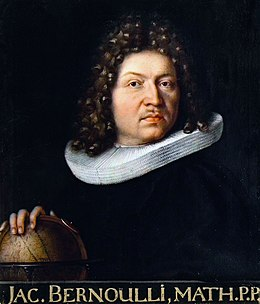
\includegraphics[width=4cm]{Jakob_Bernoulli.jpg}\\\footnotesize Jacques Bernoulli peint en 1687.}

\dleft{11cm}{
    \begin{definition}[]
        Soit $p\in\oio{0}{1}$.\\
        La loi de la  variable aléatoire $X$ donnée dans le tableau ci-contre est appelée \textbf{loi de Bernoulli de paramètre $p$}.\\
        On la note $\mathcal{B}(p)$.
    \end{definition}
}
{\tabstyle[UGLiGreen]
\begin{tabular}{|c|c|c|}
\hline
\ccell $x_i$ & $\quad 0\quad$ & $\quad 1\quad$ \\\hline
\ccell $P(X=x_i)$ & $1-p$ & $p$ \\\hline
\end{tabular}}

\begin{propriete}[]
    Soient $p\in\oio{0}{1}$ et $X$ une variable aléatoire suivant une loi de Bernoulli de paramètre $p$.\\
    On a :
    \begin{multicols}{3}
        \begin{enumerate}[label=\textbullet]
            \item $E(X)=p$
            \item $V(X)=p(1-p)$
            \item $\sigma(X)=\sqrt{p(1-p)}$
        \end{enumerate}
    \end{multicols}
\end{propriete}

\begin{demonstration}
    \begin{enumerate}[label=\textbullet]
        \item \begin{tabbing}
            $E(X)$  \=$=(1-p)\times 0+p\times 1$\\
            \>  $=p$
        \end{tabbing}
\newpage
        \item \begin{tabbing}
            $V(X)$  \=  $=(1-p)\times (0-p)^2+p\times (1-p)^2$\\
            \>  $=p^2(1-p)+p(1-p)^2$\\
            \>  $=p(1-p)(p+1-p)$\\
            \>  $=p(1-p)$
        \end{tabbing}
    \end{enumerate}
\end{demonstration}

\dleft{13.3cm}{
    \begin{exemple}
        On lance un dé équilibré.\\
        $X$ est la variable aléatoire qui prend la valeur $1$ si on obtient six au lancé de dé et $0$ sinon.\\
        $X$ suit une loi de Bernoulli de paramètre $\dfrac{1}{6}$.\\
        L'espérance de $X$ est donc $\quad E(X)=\dfrac{1}{6}$.\\[.5em]
        L'écart-type de $X$ est $\quad \sigma(X)=\sqrt{\dfrac{1}{6}\times\dfrac{5}{6}}=\dfrac{\sqrt{5}}{6}$.
    \end{exemple}
}
{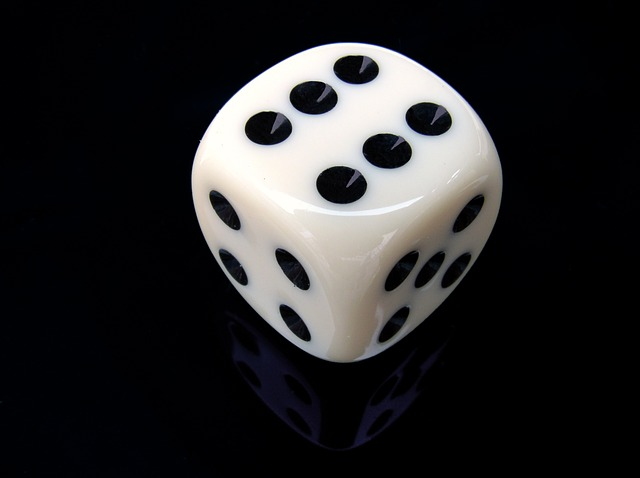
\includegraphics[width=3cm]{dice-689617_640.jpg}}


\section{Schéma de Bernoulli}
\begin{definition}[]
    Soient $n$ un entier strictement positif et $p\in\oio{0}{1}$.\\
    L'expérience aléatoire consistant à répéter $n$ fois de manière indépendante une épreuve de Bernoulli de paramètre $p$ s'appelle un \textbf{schéma de Bernoulli de paramètres $n$ et $p$}.
\end{definition}

\begin{exemple}
    On lance un dé deux fois de suite. Pour chaque lancer, le succès $S$ est l'obtenion d'une 6.\\
    Cette expérience suit un schéma de Bernoulli de paramètres $2$ et $\dfrac{1}{6}$.
    \def\abun{$S$}
    \def\alun{$\frac{1}{6}$}
    \def\abdeux{$\barmaj{S}$}
    \def\aldeux{$\frac{5}{6}$}
    \def\abtrois{$S$}
    \def\altrois{$\frac{1}{6}$}
    \def\abquatre{$\barmaj{S}$}
    \def\alquatre{$\frac{5}{6}$}
    \def\abcinq{$S$}
    \def\alcinq{$\frac{1}{6}$}
    \def\absix{$\barmaj{S}$}
    \def\alsix{$\frac{5}{6}$}
    \begin{center}
        \arbreproba
    \end{center}

    On lance un dé trois fois de suite.\\
    Cette expérience suit un schéma de Bernoulli de paramètres $3$ et $\dfrac{1}{6}$.
    \begin{center}
    \begin{tikzpicture}[
        grow=right, % Les branches poussent vers la droite
        level distance=8em, % Distance entre les niveaux
        level 1/.style={sibling distance=12em}, % Niveau 1 : distance entre nœuds
        level 2/.style={sibling distance=6em},  % Niveau 2
        level 3/.style={sibling distance=3em},  % Niveau 3
        edge from parent/.style={draw, -}, % Branches simples sans flèches
        every node/.style={align=center, font=\footnotesize} % Style des nœuds
    ]
        % Racine
        \node {} 
            % Niveau 1
            child {
                node {$\bar{S}$} % Succès au premier tirage
                child {
                    node {$\bar{S}$} % Succès au deuxième tirage
                    child {
                        node {$\bar{S}$} % Succès au troisième tirage
                        edge from parent node[below] {$\frac{5}{6}$}
                    }
                    child {
                        node {$S$} % Échec au troisième tirage
                        edge from parent node[above] {$\frac{1}{6}$}
                    }
                    edge from parent node[below] {$\frac{5}{6}$}
                }
                child {
                    node {$S$} % Échec au deuxième tirage
                    child {
                        node {$\bar{S}$} % Succès au troisième tirage
                        edge from parent node[below] {$\frac{5}{6}$}
                    }
                    child {
                        node {$S$} % Échec au troisième tirage
                        edge from parent node[above] {$\frac{1}{6}$}
                    }
                    edge from parent node[above] {$\frac{1}{6}$}
                }
                edge from parent node[below] {$\frac{5}{6}$}
            }
            child {
                node {$S$} % Échec au premier tirage
                child {
                    node {$\bar{S}$} % Succès au deuxième tirage
                    child {
                        node {$\bar{S}$} % Succès au troisième tirage
                        edge from parent node[below] {$\frac{5}{6}$}
                    }
                    child {
                        node {$S$} % Échec au troisième tirage
                        edge from parent node[above] {$\frac{1}{6}$}
                    }
                    edge from parent node[below] {$\frac{5}{6}$}
                }
                child {
                    node {$S$} % Échec au deuxième tirage
                    child {
                        node {$\bar{S}$} % Succès au troisième tirage
                        edge from parent node[below] {$\frac{5}{6}$}
                    }
                    child {
                        node {$S$} % Échec au troisième tirage
                        edge from parent node[above] {$\frac{1}{6}$}
                    }
                    edge from parent node[above] {$\frac{1}{6}$}
                }
                edge from parent node[above] {$\frac{1}{6}$}
            };
    \end{tikzpicture}
\end{center}
\end{exemple}

\section{Coefficients binomiaux}
\begin{definition}[]
    Soient $n$ un entier naturel non nul et $k$ un entier compris entre $0$ et $n$.\\
    Le \textbf{coefficient binomial} $\displaystyle\binom{n}{k}$ est le nombre de façons d'obtenir $k$ succès dans un schéma de Bernoulli de taille $n$.\\[.5em]
    $\displaystyle\binom{n}{k}$ se lit « $k$ parmi $n$ ».\\[.5em]
    Par convention, $\displaystyle\binom{0}{0}=1$.
\end{definition}

\begin{exemple}[]
    Dans l'arbre précédent représentant un schéma de Bernoulli de paramètres $3, \dfrac{1}{6}$ :
    \begin{enumerate}[label=\textbullet]
        \item Il y a un seul chemin qui comporte trois succès. Donc $\displaystyle\binom{3}{3}=1$.
        \item Il y a trois chemins qui ne comportent qu'un succès. Donc $\displaystyle\binom{3}{1}=3$.
    \end{enumerate} 
\end{exemple}

\begin{propriete}[s]
    \begin{enumerate}[label=\textbullet]
        \item $\displaystyle\binom{n}{0}=1\quad$ et $\quad\displaystyle\binom{n}{n}=1$.
        \item \textbf{Symétrie des coefficients binimiaux} : Pour tout entier $k$ tel que $0\leqslant k\leqslant n, \quad \displaystyle \binom{n}{k}=\binom{n}{n-k}$.
    \end{enumerate}
\end{propriete}

\begin{demonstration}
    Dans un arbre représentant un schéma de Bernoulli de taille $n$ :
    \begin{enumerate}[label=\textbullet]
        \item  Un seul chemin ne réalise aucun succès donc $\displaystyle\binom{n}{0}=1$ et un seul chemin réalise $n$ succès donc $\displaystyle\binom{n}{n}=1$.
        \item Il y a autant de chemins qui réalisent $k$ succès que de chemins qui réalisent $k$ échecs (c'est-à-dire $n-k$ succès).
    \end{enumerate}
\end{demonstration}

\dleft{12.8cm}{
\begin{propriete}[ - Formule de Pascal (admise)]
    Pour tous entiers naturels $n$ et $k$ tels que $n\geqslant 1$ et $0\geqslant k\geqslant n-1$, $$\displaystyle \binom{n}{k}+\binom{n}{k+1}=\binom{n+1}{k+1}.$$
\end{propriete}
}{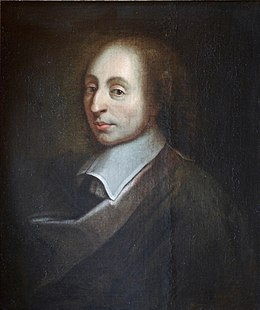
\includegraphics[width=3cm]{Blaise_Pascal_Versailles.JPG}\\
\footnotesize Blaise PASCAL en 1691}
%\newpage

\textbf{Calcul des coefficients binomiaux à l'aide du triangle de Pascal :}\\

\dleft{8.2cm}{
On peut calculer les coefficients binomiaux de proche en proche à l'aide du tableau ci-contre :
\begin{enumerate}[label=\textbullet]
    \item On convient que $\displaystyle \binom{0}{0}=1$ ;
    \item On place des $1$ sur la colonne « $k=0$ » du fait que $\displaystyle \binom{n}{0}=1$ ;
    \item On place des $1$ sur la diagonale du fait que $\displaystyle \binom{n}{n}=1$ ;
    \item On obtient nombre du tableau en additionant le nombre juste au-dessus et celui situé à gauche sur la ligne précédente, d'après la formule de Pascal.
\end{enumerate}}
{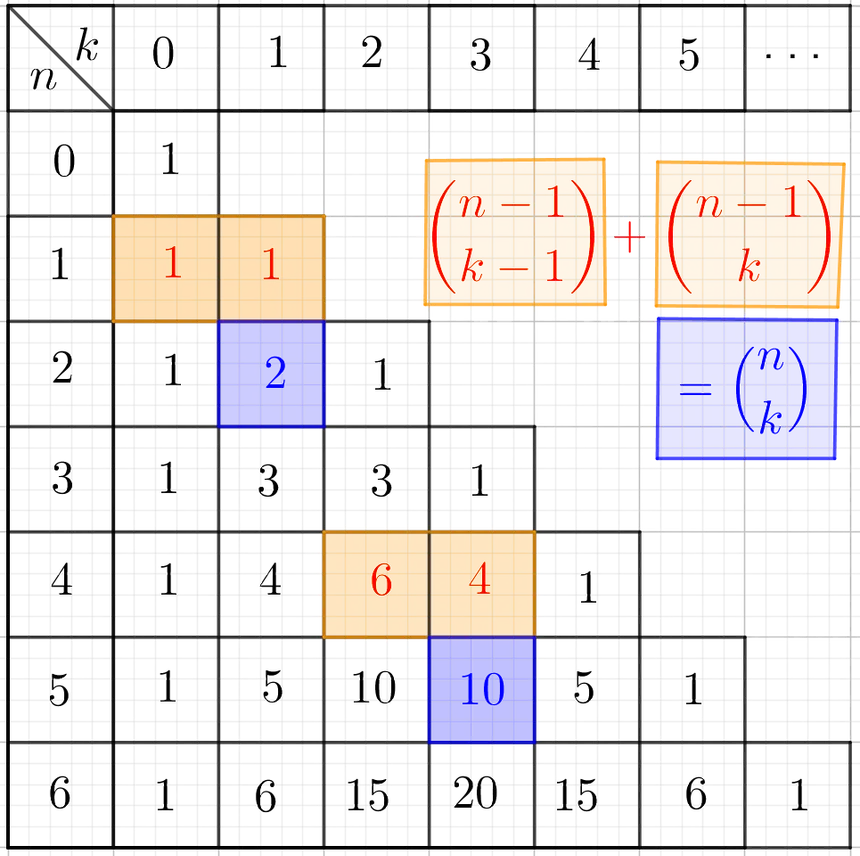
\includegraphics[width=8cm]{Triangle-de-Pascal-01-3.jpg}}


\section{Loi binomiale}
\begin{definition}[]
    Soient $n\in\N^*$ et $p\in\oio{0}{1}$.\\
    Soit $X$ une variable aléatoire qui, à chaque issue d'un schéma de Bernoulli de paramètres $n$ et $p$, associe le nombre de succès au cours de ces $n$ épreuves.\\
    La loi de probabilité de $X$ est appelée \textbf{loi binomiale de paramètres $n$ et $p$}.\\
    On la note $\mathcal{B}(n,p)$.
\end{definition}

\begin{exemple}[]
    Un QCM comporte trois questions. Pour chacune d'elles, quatre réponses sont proposées dont une seule est correcte. Un élève choisit au hasard une réponse à chaque question indépendamment des autres.\\
    La variable aléatoire $X$ compte le nombre de bonnes réponses données par l'élève.\\

    \textbf{Épreuve de Bernoulli :} Choisir au hasard une réponse à une question. Le succès est « La réponse est correcte » et $p=P(S)=\dfrac{1}{4}$.\\[.5em]
    \textbf{Schéma de Bernoulli :} On répète $n=3$ fois cette épreuve de Bernoulli dans des conditions d'indépendance.\\[.5em]
    \textbf{Loi binomiale :} La variable aléatoire $X$ suit la loi binomiale de paramètres $n=3$ et $p=\dfrac{1}{4}$.\\
    \setlength{\columnseprule}{0.5pt}
    \begin{multicols}{3}
        \begin{center}
            \textbf{Arbre pondéré}\\[1em]
            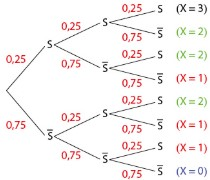
\includegraphics[width=5cm]{arbre.jpg}\\
            \vfill\null\columnbreak
            \textbf{Loi de probabilité de $X$}
        \end{center}
            À l'aide de l'arbre pondéré, on peut calculer la loi de probabilité de $X$.
        \begin{center}
            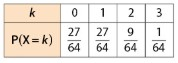
\includegraphics[width=4.5cm]{tableau.jpg}\\
            \vfill\null\columnbreak
            \textbf{Représentation graphique}
        \end{center}
            On représente la loi de probabilité de $X$ à l'aide d'un diagramme en bâtons.
        \begin{center}
            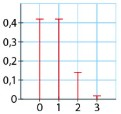
\includegraphics[width=3cm]{diagramme.jpg}
        \end{center}
    \end{multicols}
\end{exemple}

\begin{propriete}[]
    Soit $X$ une variable aléatoire suivant la loi $\mathcal{B}(n,p)$.\\
    Pour tout entier $k$ compris entre $0$ et $n$, on a $\quad P(X=k)=\displaystyle\binom{n}{k}\ p^k\ (1-p)^{n-k}$.
\end{propriete}

\begin{demonstration}
    Dans l'arbre modélisant une épreuve de Bernoulli à $n$ épreuves, l'évènement $\left\{X=k\right\}$ est formé de $\displaystyle\binom{n}{k}$ issues, car il y a $\displaystyle\binom{n}{k}$ chemins réalisant $k$ succès.\\
    Ces issues ont toutes la même probabilité $p^k\ (1-p)^{n-k}$, d'aprè une propriété des arbres pondérés.\\
    On obtient ainsi $P(X=k)=\displaystyle\binom{n}{k}\ p^k\ (1-p)^{n-k}$.
\end{demonstration}

\begin{exemple}[]
    Dans l'exemple précédent, $X$ suit une loi binomiale de paramètres $3, \dfrac{1}{4}$. 
    \begin{tabbing}
        On a : $\quad P(X=2)$    \=  $=\displaystyle\binom{3}{2}\times \left(\frac{1}{4}\right)^2\times \left(1-\frac{1}{4}\right)^{3-2}$\\[.5em]
        \>  $=3\times \dfrac{1}{16} \times \dfrac{3}{4}$\\[.5em]
        \>  $=\dfrac{9}{64}$
    \end{tabbing}   
\end{exemple}

\begin{propriete}[ (admise)]
    Si $X$ est une variable aléatoire qui suit une loi binomiale de paramètres $n$ et $p$, alors :
    \setlength{\columnseprule}{0pt}
    \begin{multicols}{3}
        \begin{enumerate}[label=\textbullet]
            \item $E(X)=np$
            \item $V(X)=np(1-p)$
            \item $\sigma(X)=\sqrt{np(1-p)}$
        \end{enumerate}
    \end{multicols}
\end{propriete}

\vspace*{.5cm}
\dleft{14cm}{
    \textcolor{UGLiBlue}{Tutoriel vidéo pour calculer des probabilités dans le cadre d'une loi binomiale à l'aide de la calculatrice :}\\
    %https://ladigitale.dev/digiview/#/v/6754c56544eb0
}
{
\includegraphics[width=2cm]{code-qr1.png}}

\subsection*{Intervalles de fluctuation et loi binomiale}

\begin{definition}[]
    Soient $X$ une variable aléatoire suivant une loi binomiale et $\alpha\in\oio{0}{1}$.\\
    Un intervalle $\fif{a}{b}$ (avec $a$ et $b$ deux réels) tel que $\quad P(a\leqslant X\leqslant b)\geqslant 1-\alpha \quad$ est appelé \textbf{intervalle de fluctuation} au seuil de $1-\alpha$ (ou au risque $\alpha$) associé à $X$. 
\end{definition}

\begin{exemple}[s]
    On considère une variable aléatoire $X$ suivant la loi $\mathcal{B}(43\ ;0,2)$ et $\alpha=0,05$ (donc $1-\alpha=0,95$).
    \begin{enumerate}
        \item On a $\quad P(X\leqslant 12) <0,95\quad$ et $\quad P(X\leqslant 13)\approx 0,964\quad $ donc $\quad P(X\leqslant 13) \geqslant 0,95$.
        \begin{center}
            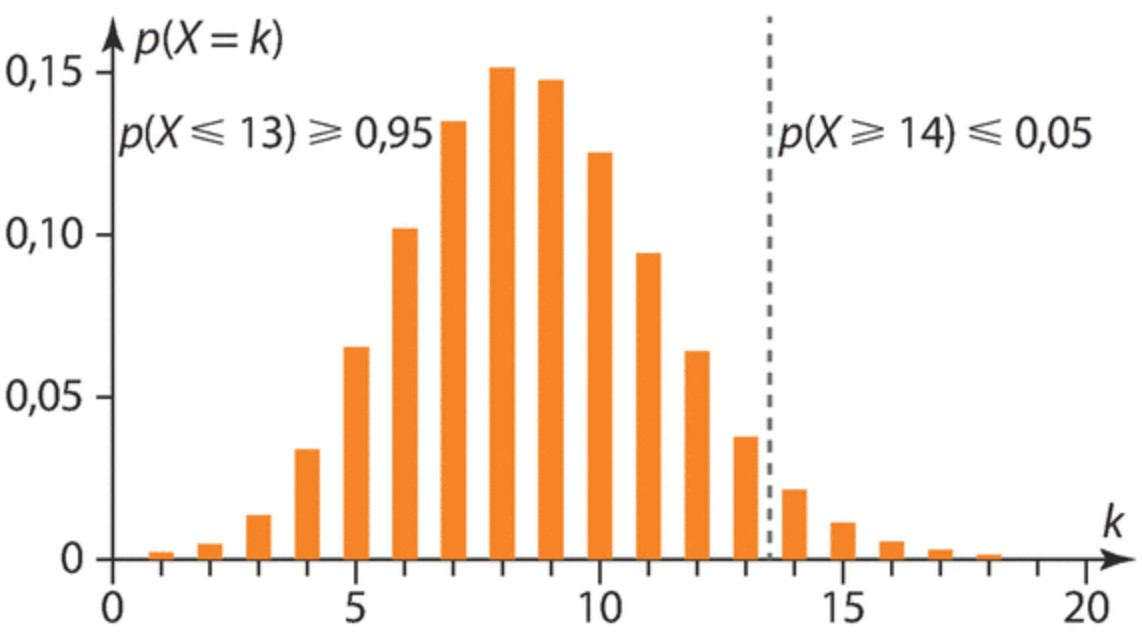
\includegraphics[width=8cm]{fluctuation1.jpg}
        \end{center}
        Ainsi $\fif{0}{13}$ est un intervalle de fluctuation au seuil de $1-\alpha=0,95$ associé à $X$ :\\[.5em]
        Pour la variable aléatoire $X$, la probabilité qu'il n'y ait pas plus de 13 succès sur les 43 répétitions est supérieure à 95 \%.
       
        \item On a $\quad \dfrac{\alpha}{2}=0,025\quad$ et $\quad 1-\dfrac{\alpha
        }{2}=0,975$.
        \begin{center}
            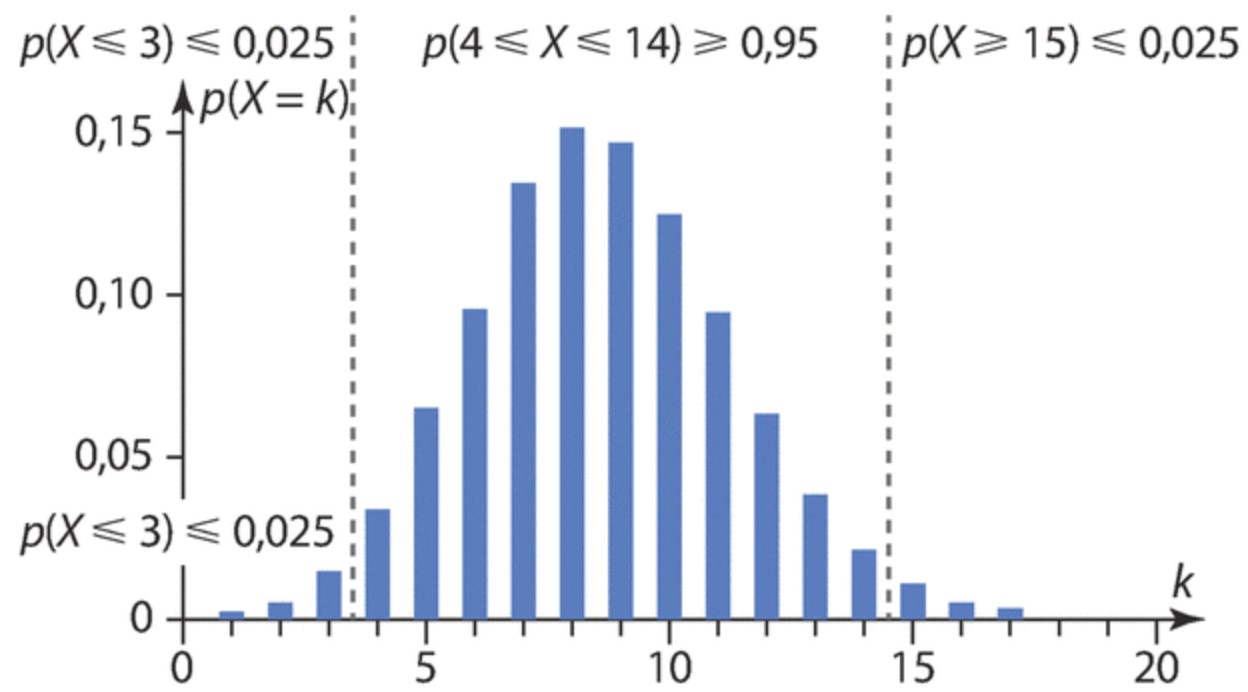
\includegraphics[width=9cm]{fluctuation2.jpg}
        \end{center}
        \begin{enumerate}[label=\textbullet]
            \item $P(X\leqslant 3)\approx0,018\leqslant 0,025\quad$ et $\quad P(X\leqslant 4)\approx0,051>0,025$.
            \item $P(X\leqslant 13)\approx0,964< 0,975\quad$ et $\quad P(X\leqslant 14)\approx0,984 \geqslant 0,975$.
        \end{enumerate}
        Ainsi $\fif{4}{14}$ est un intervalle de fluctuation centré au seuil de $1-\alpha=0,95$ associé à $X$ :\\[.5em]
        Pour la variable aléatoire $X$, la probabilité qu'il y ait entre 4 et 14 succès sur les 43 répétitions est supérieure à 95 \%.
    \end{enumerate}
\end{exemple}

\vspace*{.5cm}
\dleft{14cm}{
    \textcolor{UGLiBlue}{Tutoriel vidéo pour calculer des intervalles de confiance dans le cadre d'une loi binomiale à l'aide de la calculatrice :}\\
    %https://ladigitale.dev/digiview/#/v/6755f5a97ca26
}
{
\includegraphics[width=2cm]{code-qr2.png}}

\section{Loi géométrique}
\begin{definition}[]
    On considère une épreuve de Bernoulli pour laquelle la probabilité d'un succès est $p$.\\
    On répète cette épreuve de Bernoulli de manière indépendante jusqu'à l'obtention du premier succès.\\
    La variable aléatoire $X$ donnant le nombre d'essais nécessaires pour obtenir ce succès suit la \textbf{loi géométrique de paramètre $p$}, notée $\mathcal{G}(p)$.
\end{definition}


\begin{exemple}[]
    \dleft{13cm}{
        On lance un dé équilibré à quatre faces numérotées de 1 à 4 jusqu'à l'obtention d'un 4.\\
        La variable aléatoire $Y$ donnant le nombre d'essais nécessaires pour obtenir un 4 suit la loi géométrique de paramètre $p=0,25$ :}
        {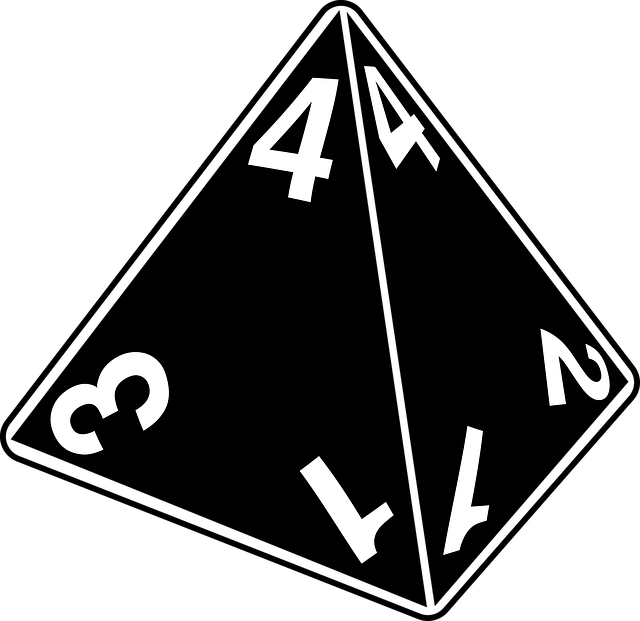
\includegraphics[width=2.3cm]{d4-die-7321725_640.png}}
        \begin{enumerate}[label=\textbullet]
            \item $Y$ donne le nombre d'essais pour obtenir un succès ;
            \item Les lancers de dés sont indépendants ;
            \item Ces lancers sont des épreuves de Bernoulli identiques de paramètre $0,25$.
        \end{enumerate}
\end{exemple}


\begin{propriete}[]
    Soient $p\in\oio{0}{1}$ et $X$ une variable aléatoire qui suit une loi géométrique de paramètre $p$.\\
    Pour tout entier naturel $k$ non nul, $\quad P(X=k)=p(1-p)^{k-1}$.
\end{propriete}


\dleft{10cm}{
    \begin{demonstration}
        On répète $k$ fois une épreuve de Bernoulli telle que $P(S)=p$.\\
        L'évènement $\left\{X=k\right\}$ est réalisé lorsque l'on obtient $k-1$ échecs suivi d'un succès.\\
        Donc $P(X=k)=(1-p)^{k-1}\times p$.
    \end{demonstration}
}
{
    \begin{tikzpicture}[
        grow=right, % Les branches poussent vers la droite
        level distance=6em, % Distance entre les niveaux
        level 1/.style={sibling distance=6em}, % Niveau 1 : distance entre nœuds
        level 2/.style={sibling distance=4em},  % Niveau 2
        level 3/.style={sibling distance=2em},  % Niveau 3
        edge from parent/.style={draw, -}, % Branches simples sans flèches
        every node/.style={align=center, font=\footnotesize} % Style des nœuds
    ]
        % Racine
        \node {} 
            % Niveau 1
            child {
                node {$\bar{S}$} % Echec au premier tirage
                child {
                    node {$\bar{S}\ ...$} % Echec au deuxième tirage
                    edge from parent node[below] {$1-p$}
                }
                child {
                    node {$S$} % Succès au deuxième tirage
                    edge from parent node[above] {$p$}
                }
                edge from parent node[below left] {$1-p$}
            }
            child {
                node {$S$} % Succès au premier tirage
                edge from parent node[above] {$p$}
            };
    \end{tikzpicture}
}

\begin{propriete}[ (admise)]
    Soient $p\in\oio{0}{1}$ et $X$ une variable aléatoire qui suit la loi géométrique de paramètre $p$.\\
    L'espérance de $X$ est $\quad E(X)=\dfrac{1}{p}$.    
\end{propriete}

\begin{exemple}[]
    Dans l'exemple précédent, $Y$ suit la loi $\mathcal{G}(0,25)$ donc la probabilité qu'il faille cinq essais pour obtenir un 4 est :
    \begin{tabbing}
        $P(Y=5)$    \=  $(1-0,25)^{5-1}\times 0,25$\\
        \>  $=0,75^4\times 0,25$\\
        \>  $\approx 0,08$
    \end{tabbing} 
    L'espérance de $Y$ est $\quad E(Y)=\dfrac{1}{0.25}=4$.\\
    Cela signifie que si l'on recommence un grand nombre de fois cette succession d'épreuves, alors le nombre moyen d'essais à réaliser afin d'obtenir un 4 est proche de quatre.
\end{exemple}


\dleft{10cm}{
    \subsection*{Représentation graphique d'une loi géométrique}
    Pour $X$, variable aléatoire suivant la loi $\mathcal{G}(p)$, son diagramme en barres associé correspond à une décroissance exponentielle et $p=P(X=1)$ est la hauteur de la première barre.
}
{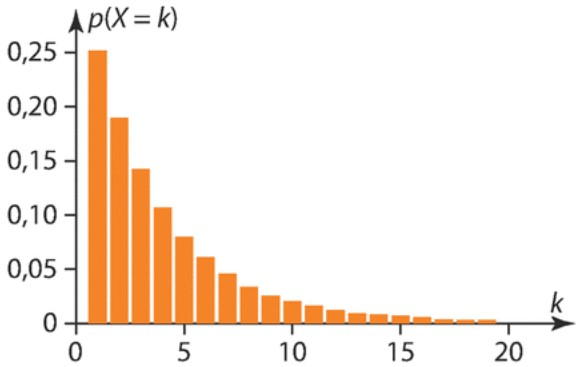
\includegraphics[width=6cm]{diagramme_geom.jpg}}

\subsection*{Absence de mémoire de la loi géométrique}
\begin{propriete}[]
    Soient $p\in\oio{0}{1}$ et $X$ une variable aléatoire qui suit la loi géométrique de paramètre $p$.\\
    Pour tout entier $k$ strictement positif, $\quad P(X>k)=(1-p)^k$.
\end{propriete}

\begin{demonstration}
    Soit $X$ une variable aléatoire suivant une loi géométrique de paramètre $p$.
    \begin{tabbing}
        $P(X>k)$    \=$=1-P(X\leqslant k)$\\[.5em]
        \>  $=1-\left[P(X=1)+...+P(X=k)\right]$\\[.5em]
        \>  $=1-\left[p+p(1-p)+...+p(1-p)^{k-1}\right]$\\[.5em]
        \>  $=1-p\left(1+(1-p)+...+(1-p)^{k-1}\right)$\\[.5em]
        \>  $=1-p\ \dfrac{1-(1-p)^k}{1-(1-p)}$\\[.5em]
        \>  $=1-p\ \dfrac{1-(1-p)^k}{p}$\\[.5em]
        \>  $=1-\left(1-(1-p)^k\right)$\\[.5em]
        \>  $=(1-p)^k$
    \end{tabbing}
\end{demonstration}

\begin{propriete}[]
    Soit $X$ une variable aléatoire à valeurs dans $\N^*$.
    \begin{enumerate}[label=\textbullet]
        \item Si $X$ suit une loi géométrique, alors pour tous $k\in\N^*$ et $n\in\N^*$,\\ $P_{X>n}(X>k+n)=P(X>k)$.
        \item Réciproquement, si pour tous $k\in\N^*$ et $n\in\N^*$, $\quad P_{X>n}(X>k+n)=P(X>k), \quad$ alors $X$ suit une loi géométrique.
    \end{enumerate}
\end{propriete}

\begin{demonstration}
    Démonstration du premier point :\\
    Soit $X$ une variable aléatoire suivant une loi géométrique de paramètre $p$.
        \begin{tabbing}
            $P_{X>n}(X>k+n)$    \=  $=\dfrac{P\left(\left\{X>k+n\right\}\cap \left\{X>n\right\}\right)}{P(X>n)}$\\[.5em]
            \>  $=\dfrac{P(X>k+n)}{P(X>n)}$\\[.5em]
            \>  $=\dfrac{(1-p)^{k+n}}{(1-p)^n}$\\[.5em]
            \>  $=(1-p)^k$\\[.5em]
            \>  $=P(X>k)$
        \end{tabbing}
\end{demonstration}





\end{document}